\let\negmedspace\undefined
\let\negthickspace\undefined
\documentclass[journal]{IEEEtran}
\usepackage[a5paper, margin=10mm, onecolumn]{geometry}
%\usepackage{lmodern} % Ensure lmodern is loaded for pdflatex
\usepackage{tfrupee} % Include tfrupee package

\setlength{\headheight}{1cm} % Set the height of the header box
\setlength{\headsep}{0mm}     % Set the distance between the header box and the top of the text

\usepackage{gvv-book}
\usepackage{gvv}
\usepackage{cite}
\usepackage{amsmath,amssymb,amsfonts,amsthm}
\usepackage{algorithmic}
\usepackage{graphicx}
\usepackage{textcomp}
\usepackage{xcolor}
\usepackage{txfonts}
\usepackage{listings}
\usepackage{enumitem}
\usepackage{mathtools}
\usepackage{gensymb}
\usepackage{comment}
\usepackage[breaklinks=true]{hyperref}
\usepackage{tkz-euclide} 
\usepackage{listings}
% \usepackage{gvv}                                        
\def\inputGnumericTable{}                                 
\usepackage[latin1]{inputenc}                                
\usepackage{color}                                            
\usepackage{array}                                            
\usepackage{longtable}                                       
\usepackage{calc}                                             
\usepackage{multirow}                                         
\usepackage{hhline}                                           
\usepackage{ifthen}                                           
\usepackage{lscape}
\begin{document}

\bibliographystyle{IEEEtran}
\vspace{3cm}

\title{1-1.4-9l}
\author{AI24BTECH11028- Ronit Ranjan}

% \maketitle
% \newpage
% \bigskip
{\let\newpage\relax\maketitle}

\renewcommand{\thefigure}{\theenumi}
\renewcommand{\thetable}{\theenumi}
\setlength{\intextsep}{10pt} % Space between text and floats


\numberwithin{equation}{enumi}
\numberwithin{figure}{enumi}
\renewcommand{\thetable}{\theenumi}

\textbf{Question}: \\
Find the coordinates of the point which divides the line segement joining the points (-2, 3, 5) and (1, -4, 6) in the ratio\\
i) 2:3 internally\\
ii) 2:3 externally

\textbf{Solution}: For internal divison we have,\\
\begin{align}
    D = \frac{kC + B}{k + 1}
\end{align}
Here $C = \brak{1, -4, 6}$, $B = \brak{-2, 3, 5}$ and $k = \frac{2}{3}$\\
Now, Putting values in the equation we get,
\begin{figure}[hbt!]
		\centering
		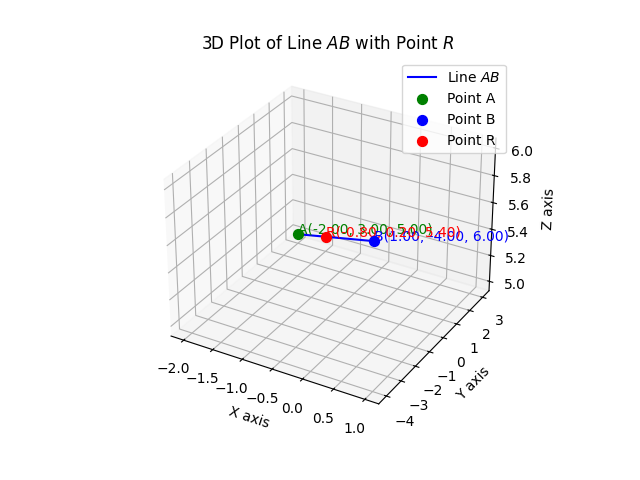
\includegraphics[width=0.6\linewidth]{plots/plot1.png}

	\end{figure}
\begin{align}
D = \frac{\frac{2}{3}
 \myvec{
   1
   \\
   -4
   \\
   6
 }
 +
 \myvec{
   -2
   \\
   3 
   \\
   5
 }}{\frac{2}{3}+1}
 \\
 D = \frac{
  \myvec{
  \frac{-4}{3}
  \\
  \frac{1}{3}
  \\
  9
  }
  }{\frac{5}{3}}
  \\
D = 
 \myvec{
  \frac{-4}{5}
  \\
  \frac{1}{5}
  \\
  \frac{27}{5}
 }
 \end{align}
 
So, the point which divides the line segement joining the points \brak{2, 3, 5} and \brak{1, -4, 6} is \brak{\frac{-4}{5}, \frac{1}{5}, \frac{27}{5}}



For external divison we have,
\begin{align}
    D = \frac{kC - B}{k - 1}
\end{align}
 \begin{figure}[hbt!]
		\centering
		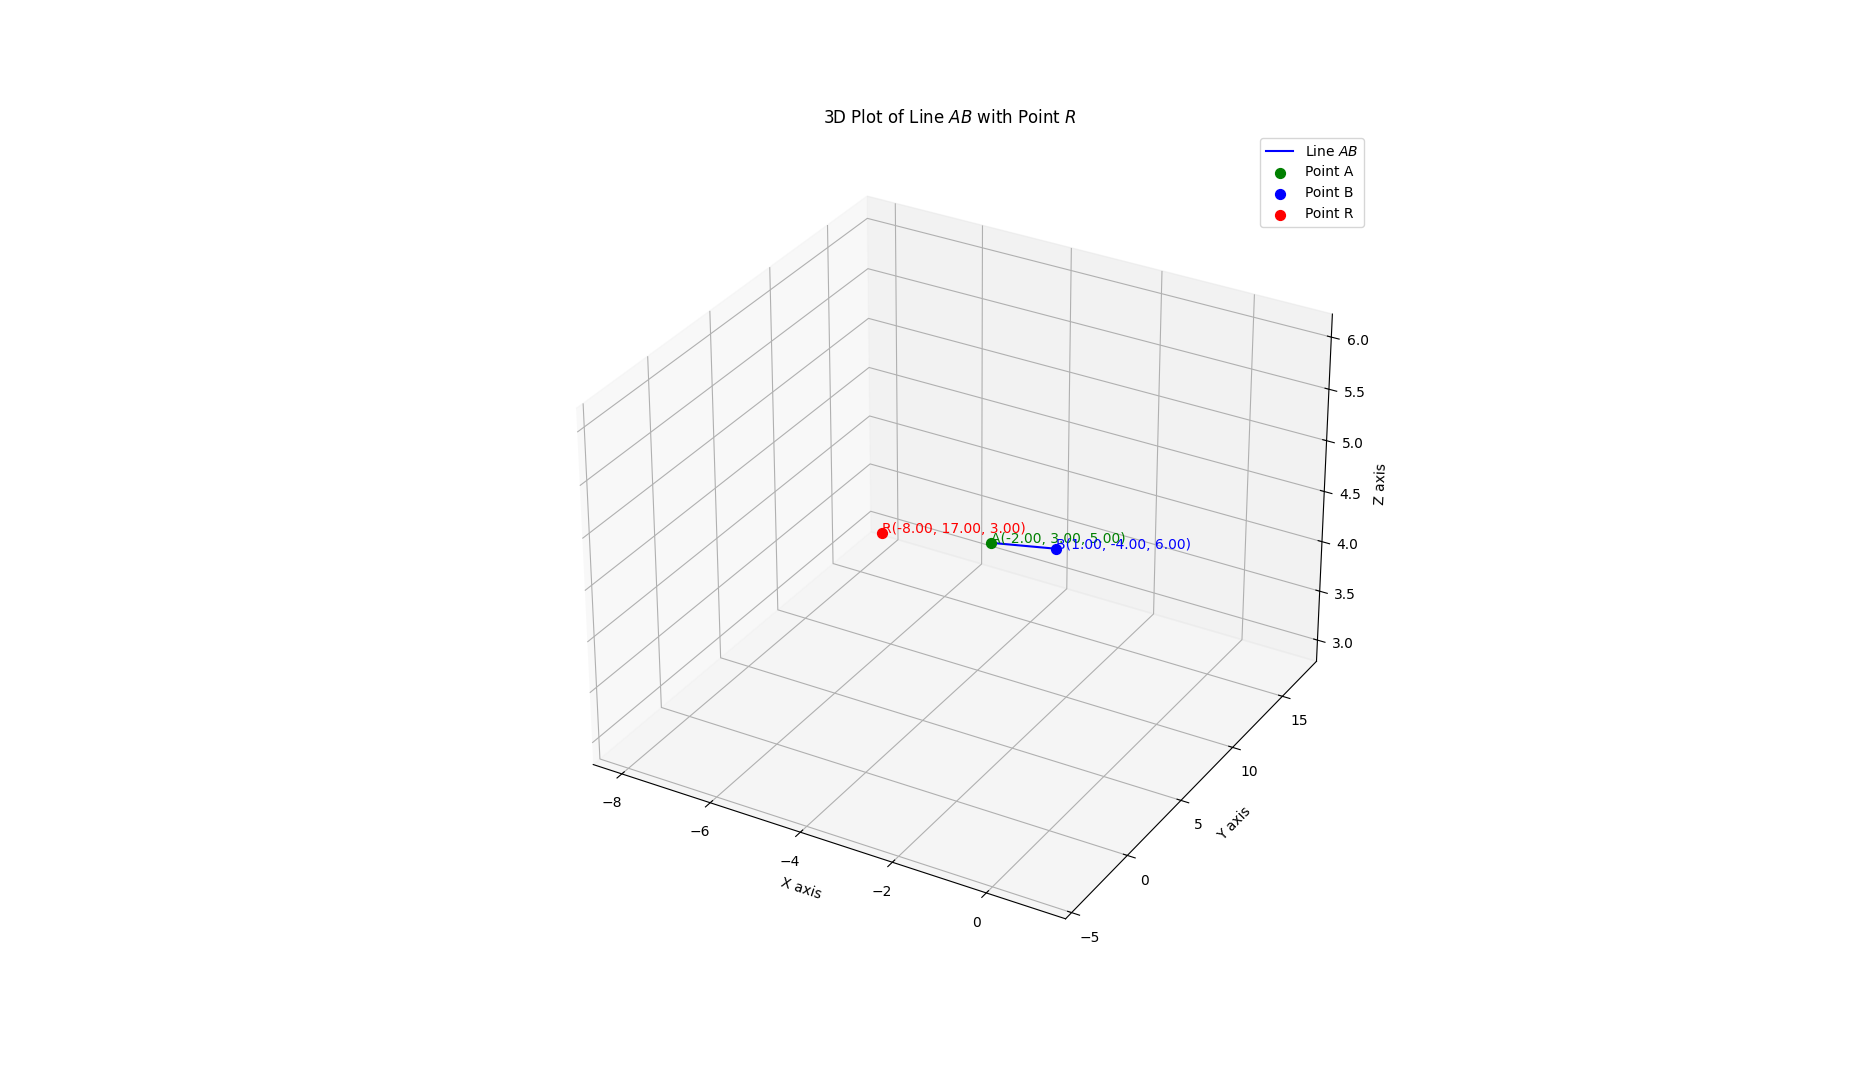
\includegraphics[width=0.8\linewidth]{plots/plot2.png}

	\end{figure}
Now, Putting values in the equation we get,
\begin{align}
D = \frac{\frac{2}{3}
 \myvec{
   1
   \\
   -4
   \\
   6
 }
 -
 \myvec{
   -2
   \\
   3 
   \\
   5
 }}{\frac{2}{3}-1}
 \\
 D = \frac{
  \myvec{
  \frac{8}{3}
  \\
  \frac{-35}{3}
  \\
  -1
  }
  }{\frac{-1}{3}}
  \\
D = 
 \myvec{
  -8
  \\
  17
  \\
  3
 }
 \end{align}
So, the point which divides the line segement joining the points \brak{2, 3, 5} and \brak{1, -4, 6} is \brak{-8, 17, 3}


\end{document}
